\section{Data Acquisition}

%head
The following section will include a description on how the data for the study have been acquired and processed. All data processing, along with GUI design and implementation, will be done in Matlab.

%presentaion of training GUI
To acquire data a training GUI has been designed and implemented in Matlab. The GUI has been designed to fulfil the specific needs for this project. An illustration of the GUI can be seen in \figref{fig:GUI_Training}. 

\begin{figure}[H]
	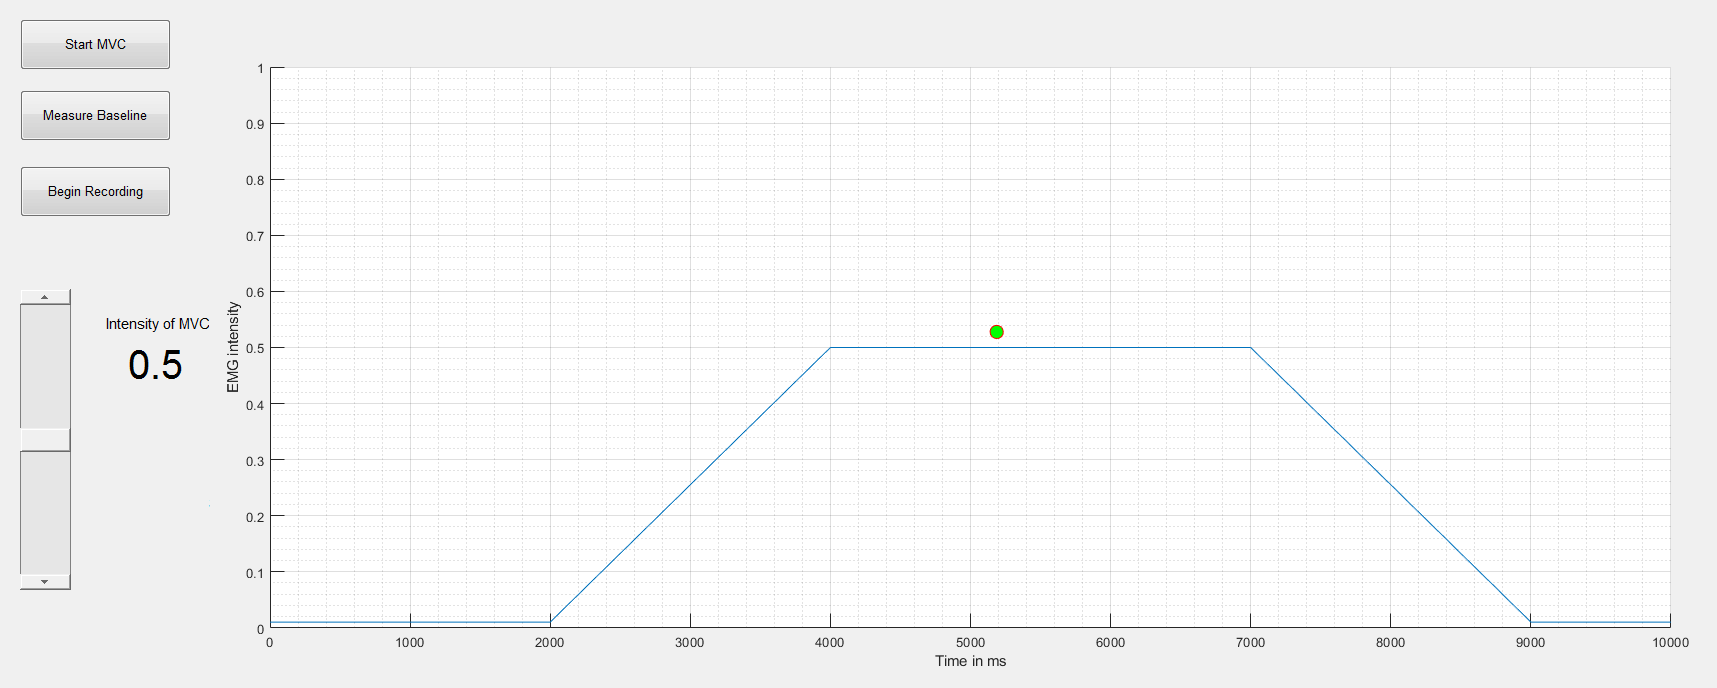
\includegraphics[width=.4\textwidth]{figures/GUI/GUI_Training.png}
	\caption{\textbf{WE GONNA NEED A NEW PIC OF THE GUI HERE} The training GUI implemented with Matlab GUI development environment. Control buttons to calculate MVC and perform MVC fraction recordings are placed on the left side. The trapezoid plot with the green dot controlled by the input EMG signal from the subject is shown on the right. The fraction of the MVC can be defined by the slider located under the control buttons.}
	\label{fig:GUI_Training}
\end{figure} 

The functions of the GUI consists of a baseline measurement button, a MVC measurement button, a data recording button and a fraction of MVC intensity slider. The baseline measurement is acquired for the purpose of being subtracted from the signal, in order to remove the signal artefacts that are present. At the baseline acquisition the subject is resting the lower arm in the given limb position. The MVC is calculated as a mean of the maximum values in each of the eight channels, and is set as a normalized reference point of 1. The MVC is a contraction at the intensity of which the subject can withhold for 15 seconds. The data recording contains the raw data of a given fraction of the MVC. The fraction is decided by setting the slider to the wanted fraction value, before the recording is started. The slider sets the fraction value so the plateau of the trapeze is at the set value. The trapeze depicts an initial resting phase of two seconds with the intensity of 0, a transition phase of two seconds with an ascending slope until the plateau phase is reached, which has a three second duration, and then a final descending transition phase of two seconds and resting phase of one second. Initialization of the recording will show a green dot, which moves with time in relation to the normalized intensity. The green dot is calculated as the mean of the input EMG signal in a 200 ms window with a 100 ms overlap. %The signal is afterwards normalized with the MVC measurement as the reference point. 
From this acquired data features will be extracted and used to train regressors for each of the subjects for each of the hand gestures performed.


\subsection{Validation of data}

%collect data (described earlier)
%review data to evaluate if the acquired data is valid for training the regressors
%do PCA to validate data (qualitatively) -> t-test (only later if we are fast) to check if data clouds are significalnty different from each other
%if data is different: good. if data not different: bad, redo data acquisition
%do training of regressors (next section)

After features has been extracted from the data, the feature data is validated through Principal Component Analysis (PCA) to determine the quality of the recorded data in the sense of identify outliers and examining whether the data from the different hand gestures are distinguishable. Thus, the PCA will only be used as a qualitative tool to validate the data. %due to lack of time
%include if we are fast
%and t-test to decide if there are any significant outliers and if the features are significantly different from feature data of other movements. The PCA is used to determine the relation between the feature data and identifying data outliers. 
%What is PCA?
PCA is an analysis tool used to express a set of correlated variables into non-correlated components, such that the dataset can be expressed using less variables, however more defining variables for the given data set. These variables are called the principal components. Each PC is orthogonal on the former, meaning that they each define the largest variance in an axis, different from axes described by other components. PCA also provides knowledge on which components are the most defining for the data set, so only the most important can be considered. When performing PCA it provides the coefficients of the principal components (PCC), which can be visualised in a plot. This plotting of the coefficients are what is used to evaluate the quality of the feature data. A threshold of 90\% for preserved information is used. 

PCA is performed for each movement in each limb position and plotted in a three dimensional space. If the PCC's of a movement has significant outliers, or the points are clustered, it will be identified shortly after the feature extraction, and a new recording session for the test subject can be executed to prevent inaccurate training of regressors and time delays. If the data is of high quality, meaning the data points are easily distinguishable from each other, it can be used further on to train the regressors.

\begin{figure}[H]
	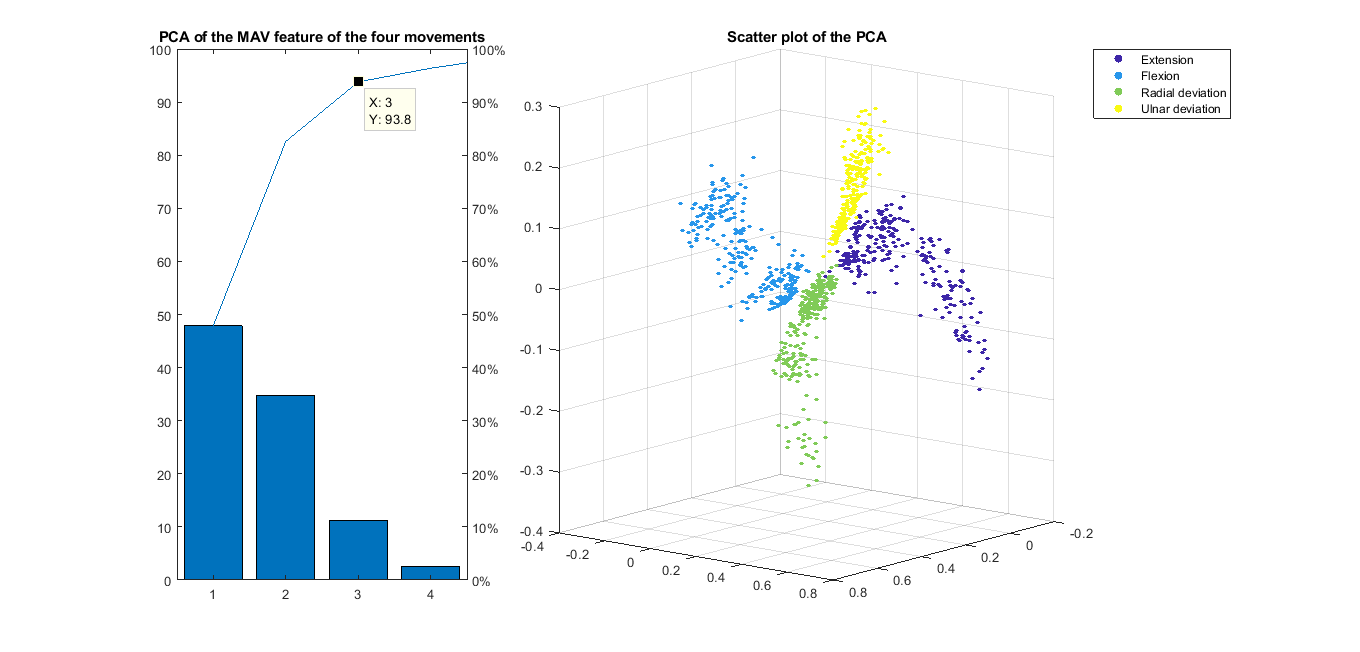
\includegraphics[width=.4\textwidth]{figures/Methods/pcasubplot.png} 
	\caption{Plot of PCA. To the left the first four principal components are visualised. The first three principal components account for describing $93.8\%$ of the data set. On the right the PCC's are plotted for each movement. The clusters for each movement are distinguishable from each other and have no noteworthy outliers, so the data is considered of high quality.} 
	\label{fig:pcasubplot}
\end{figure} 

In \figref{fig:pcasubplot} an example of a PCA performed on feature data from one test subject is shown. The left plot of the principal components describe the importance of each identified components, and how much of the variance in the data that is described. Using only the first three components, $93.8\%$ of the full dataset can be described. Only these principal components are used in the plot to the right in \figref{fig:pcasubplot}. Here it can be seen that the clusters are easily distinguishable and have no remarkable outliers. Therefore the data is considered good and can be used in the training of the regressors. 


\section{Accuracy of regressors}
To measure the accuracy of the regressors the Root Mean Squared Error(RMSE) is calculated. RMSE is a measure to examine how much the regressors disagrees with the actual data. RMSE a calculation of the standard deviation of the residuals, which is the difference between the estimated values and the actual values. The RMSE is calculated as follows:

\begin{equation}
$RMSE = \sqrt{\frac{\sum\limits_{i=1}^N(y_i - \hat{y_i})^2}{N}}
\end{equation}

Where N is the length of the signal, $y_i$ is the $i^th$ variable of the actual data and $\hat{y_i}$ is the $i^th$ output of the regressor. The RMSE will be done for the regressor for each movement. 


